\section{Laplace Transform}

Laplace transform of a function $F(t)$ denoted by $\mathcal{L}\{F(t)\}$. The Laplace operator $\mathcal{L}$ is linear, so

\begin{equation*}
    \mathcal{L}\{c_1f_1(t)+c_2f_2(t)\}=c_1\mathcal{L}\{f_1(t)\}+c_2\mathcal{L}\{f_2(t)\}
\end{equation*}

Defined as

\begin{equation*}
    \mathcal{L}\{F(t)\}=\int_0^\infty e^{-st}F(t)dt
\end{equation*}

Integral is a function of parameter $s$, say $f(s)$ such that $\mathcal{L}\{F(t)\}=f(s)$.
Improper integral will always converge, and can be written as a limit definition:

\begin{equation*}
    \int_0^\infty e^{-st}F(t)dt=\lim_{A\to \infty}\int_0^Ae^{-st}F(t)dt
\end{equation*}

We can derive some general forms based on this idea.

\subsection{Laplace transform definitions}

\begin{definition}($\mathcal{L}\{e^{kt}\}$)\\
    Finding $\mathcal{L}\{e^{kt}\}$ for $s>k$ (condition for convergence), we see that 

    \begin{equation*}
        \mathcal{L}\{e^{kt}\}=\lim_{A\to\infty} \int_0^A e^{-st}e^{kt}dt=\lim_{A\to\infty}\frac{1}{k-s}e^{(k-s)t}\mbox{$\mathcal{L}$\Large$\mid$}_0^A=\frac{1}{s-k}
    \end{equation*}
\end{definition}

\begin{definition}($\mathcal{L}\{\sin kt\}$)\\
    Evaluating the integral:
    \begin{align*}
        \int e^{-st}\sin kt&=-\frac{1}{k}e^{-st}\cos kt-\int se^{-st}\frac{1}{k}\cos kt \;dt\\
        &=-\frac{1}{k}e^{-st}\cos kt-\frac{s}{k}\int e^{-st}\cos kt \;dt\\
        &=-\frac{1}{k}e^{-st}\cos kt-\frac{s}{k}\left( \frac{1}{k}e^{-st}\sin kt-\int -\frac{s}{k}e^{-st}\sin kt\;dt \right)\\
        &=-\frac{1}{k}e^{-st}\cos kt-\frac{s}{k}\left(\frac{1}{k}e^{-st}\sin kt + \int \frac{s}{k}e^{-st}\sin kt\;dt\right)\\
        (1+\frac{s^2}{k^2})\int e^{-st}\sin kt&=-\frac{1}{k}e^{-st}\cos kt-\frac{s}{k^2}e^{-st}\sin kt\\
        \frac{k^2+s^2}{k^2}\int e^{-st}\sin kt&=\frac{1}{k}e^{-st}\cos kt-\frac{s}{k^2}e^{-st}\sin kt\\
        \int e^{-st}\sin kt&=-\frac{ke^{-st}\cos kt}{k^2+s^2}-\frac{se^{-st}\sin kt}{k^2+s^2}\\
        &=-\frac{e^{-st}}{k^2+s^2}\left(k\cos kt-s\sin kt\right)
    \end{align*}

    So evaluating the improper integral,
    
    \begin{align*}
        \left[-\frac{e^{-st}}{k^2+s^2}\left(k\cos kt-s\sin kt\right)\right]_0^\infty&=0+\frac{1(k-0)}{s^2+k^2}\\
        &=\frac{k}{s^2+k^2}
    \end{align*}

    It can be similarly obtained that $\mathcal{L}\{\cos kt\}=\frac{s}{s^2+k^2}$ (for $s>0$ in both cases).
\end{definition}

\begin{definition}($\mathcal{L}\{t\}$)
    \begin{align*}
        \mathcal{L}\{t\}&=\int_0^\infty e^{-st}tdt\\
        &=\lim_{A\to\infty}\int_0^A\underbrace{e^{-st}}_{dv}\underbrace{t}_{u}dt\\
        &=\lim_{A\to\infty}\left[ -\frac{1}{s}e^{-st}t\bigg\rvert_0^A-\int_0^A -\frac{1}{s}e^{-st}dt \right]\\
        &=\lim_{A\to\infty}\left[-\frac{1}{s}e^{-st}t-\frac{1}{s^2}e^{-st}\right]_0^A\\
        &=-\left[-\frac{1}{s^2}\right]=\frac{1}{s^2}
    \end{align*}
\end{definition}

\begin{definition}($\mathcal{L}\{\sin^2 at\}$)
    \begin{align*}
        \mathcal{L}\{\sin^2 at\}&=\mathcal{L}\{\frac{1}{2}(1-\cos 2at)\}=\frac{1}{2}\mathcal{L}\{1\}-\frac{1}{2}\mathcal{L}\{\cos 2at\}
    \end{align*}
\end{definition}

\begin{definition}(Transforms of Derivatives)
    If $F(t)$ is continuous for $t\geq 0$ and of exponential order as $t\to \infty$, then we can simplify

    \begin{align*}
        \mathcal{L}\{F'(t)\}&=\int_0^\infty e^{-st}F'(t)\;dt\\
        &=\left[e^{-st}F(t)\right]_0^\infty+s\int_0^\infty e^{-st}F(t)\;dt\\
        &=-F(0)+s\mathcal{L}\{F(t)\}
    \end{align*}

    Useful fact that can be resubstituted for \[\mathcal{L}\{F''(t)\}=-F'(0)+s\mathcal{L}\{F'(t)\}=-F'(0)-sF(0)+s^2\mathcal{L}\{F(t)\}.\]

    General form:

    \begin{equation*}
        \mathcal{L}\{f^n(t)\}=s^n\mathcal{L}\{f(t)\}-s^{n-1}f(0)-s^{n-2}f'(0)-s^{n-3}f''(0)-\ldots-f^{n-1}(0)
    \end{equation*}
\end{definition}

\begin{definition}(Translation property)
    \begin{equation*}
        \mathcal{L}\{e^{at}f(t)\}=\int_0^\infty e^{-st}e^{at}f(t)dt=\int_0^\infty e^{-(s-a)t}f(t)dt=F(s-a)
    \end{equation*}
\end{definition}

\begin{definition}($\mathcal{L}\{t^nf(t)\}$)
    \begin{align*}
        \mathcal{L}\{t^nf(t)\}=(-1)^n\frac{d^n}{ds^n}\mathcal{L}\{f(t)\}
    \end{align*}    
\end{definition}

\subsection{Solving DEs}

Approach to solving DEs involves applying Laplace to both sides of some DE

\begin{equation*}
    F(y)=f(t)
\end{equation*}

and isolating $Y(s)=\mathcal{L}\{y(t)\}$ using the derivative transform. Then, use
the inverse Laplace transform and linearity property to find $y(t)$ from $Y(s)$.

\subsection{Step Function}

\begin{figure}[H]
    \centering
    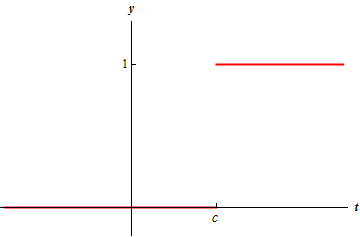
\includegraphics[scale=.5]{figures/unitstep.png}
    \caption{Unit step function}
\end{figure}

The unit step function centered at $a$ is defined as

$$
u_a(t)=u(t-a)=\begin{cases}
    0,t<a\\
    1,t\leq a
\end{cases}
$$

Can define rectangular step function with pulse width $b-a$ where $b>a$:

\begin{equation*}
    r(t)=u(t-a)-u(t-b)
\end{equation*}

Calculating the Laplace transform is simple:

\begin{align*}
    \mathcal{L}\{u_a(t)\}&=\int_0^a e^{-st}(0)dt + \int_a^\infty e^{-st}dt\\
    &=-\frac{e^{-st}}{s}\bigg\vert_a^\infty=\frac{e^{-sa}}{s}
\end{align*}

\begin{definition}(Step Function Translation)

    Let there be some arbitrary curve $f(t)$ defined for all $t$ and the step function $u(t-a)$.
    The new function $u(t-a)f(t-a)$ gives the step function with shape $f(t-a)$ for $t>a$. Applying the Laplace transform, we get

    \begin{align*}
        \mathcal{L}\{u(t-a)f(t-a)\}&=\int_0^\infty e^{-st}u(t-a)f(t-a)dt\\
        &=\int_0^a e^{-st}(0)dt+\int_a^\infty e^{-st}f(t-a)dt\\
    \end{align*}

    Let $x=t-a\implies t=x+a$. Further note that when differentiating, $dx=dt$, making this substitution useful.

    \begin{align*}
        \int_0^a e^{-st}(0)dt+\int_a^\infty e^{-st}f(t-a)dt&=\int_a^\infty e^{-s(x+a)}f(x)dt\\
        &=e^{-sa}\int_a^\infty e^{-sx}f(x)dx\\
        &=e^{-sa}\mathcal{L}\{f(t)\}
    \end{align*}
\end{definition}

\subsection{Periodic Functions}

\begin{definition} (Periodic Laplace Transform)
    If $f(t)$ is periodic, then $f(t-P)=f(t)$ (for $t\geq P$) and
    \begin{equation}
        \mathcal{L}\{f(t)\} = \displaystyle\frac{\int_0^Pe^{-st}f(t)dt}{1-e^{-Ps}}
    \end{equation}
\end{definition}

\begin{proof}
    We can write the transform as two integrals,
    \begin{align}
        F(s)&=\int_0^P e^{-st}f(t)dt + \int_P^\infty e^{-st}f(t)dt\\
        &= \int_0^P e^{-st}f(t)dt + \int_P^\infty e^{-st}f(t+P)dt\label{split}
    \end{align}

    Note that $\tau = t-P\implies t=\tau +P$ so $dt = d\tau$.
    \begin{align}
        \int_P^\infty e^{-st}f(t+P)dt &= \int_{2P}^\infty e^{-s(\tau + P)}f(\tau)d\tau\\
        &= e^{-sP}\int_{0}^\infty e^{-s\tau}f(\tau)d\tau\\
        &= e^{-sP}F(s)
    \end{align}
    Substituting into \ref{split}, we get
    \begin{equation}
        F(s)=\int_0^P e^{-st}f(t)dt + e^{-st}F(s)\implies (1-e^{-sP})F(s)=\int_0^P e^{-st}f(t)dt
    \end{equation}
\end{proof}

\subsection{Convolution Operation}

\begin{definition} (Convolution Theorem)
    \begin{equation}
        f * g = \int_0^t f(r) g(t-r)dr=g * f
    \end{equation}
    Applying the Laplace operator,
    \begin{equation}
        \mathcal{L}\{f*g\}=\mathcal{L}\{f(t)\}\mathcal{L}\{g(t)\}=F(s)G(s)
    \end{equation}
    A more useful property is of the inverse,
    \begin{equation}
        f*g=\mathcal{L}^{-1}\{F(s)G(s)\}
    \end{equation}
\end{definition}

\begin{example}
    Finding the the inverse transform, we can apply the Laplace convolution definition,
    \begin{align*}
        \mathcal{L}^{-1}\left\{\frac{a}{s^2(a^2+s^2)}\right\}&=\int_0^t (t-u)\sin au\,du\\
        &=t\int_0^t \sin au\, du -\int_0^t u\sin au\, du\\
        &=-t(\cos at - 1)-\left(-u\cos au\bigg\vert_0^t+\int_0^t \cos au\,du\right)\\
        &=t(1-\cos at)+t\cos at+\sin at
    \end{align*}
\end{example}

\subsection{More on Step Functions}

\begin{definition} (Step function)
    \begin{equation}
        \alpha(t)=\begin{cases}
            0,\;t\leq 0\\
            1,\;t>0
        \end{cases}
    \end{equation}
    \begin{figure}[H]
        \centering
        \begin{tikzpicture}
            \draw[thick, black] (-3,0)--(3,0) node[right]{$t$};
            \draw (0,0) node[below left]{$O$};
            \draw[thick, black] (0,-3)--(0,3) node[above]{$y$};
            \draw[ultra thick, color=red!70] (-3,0)--(0,0);
            \draw[ultra thick, color=red!70] (0,1) node[left] {$1$} (0,1)--(3,1);
        \end{tikzpicture}
        \caption{Unit step function}
    \end{figure}
    We can apply this to a function $F(t)$ such that $y=\alpha(t-c)F(t)$
    turns off $F$ for $t\leq c$.
\end{definition}

Applying the Laplace transform and the substitution $t-c=v$ (note that the lower bound changes from $c$ to $0$), we get

\begin{align*}
    \mathcal{L}\left\lbrace \alpha(t-c)f(t-c) \right\rbrace&=\int_0^\infty e^{-st}\alpha(t-c)f(t-c)\,dt\\
    &=\int_c^\infty e^{-st}f(t-c)\,dt\\
    &=\int_0^\infty e^{-s(c+v)}f(v)dv\\
    &=e^{-sc}\int_0^\infty e^{-sv}f(v)dv\\
    &=e^{-sc}F(s)
\end{align*}

\begin{example}
    We want to model the function
    $$y(t)=\begin{cases}
        t^2,\, 0<t<2\\
        2,\,t>2
    \end{cases}$$
    \begin{figure}[H]
        \centering
        \begin{tikzpicture}
            \draw[thick, black] (-3,0)--(3,0) node[right]{$t$};
            \draw (0,0) node[below left]{$O$};
            \draw[thick, black] (0,-3)--(0,3) node[above]{$y$};
            \draw[ultra thick, color=red!70, domain=0:2, variable=\x] plot({\x}, {\x * \x});
            \draw[dashed] (2,4)--(2,2);
            \draw[ultra thick, color=red!70] (2,2)--(3,2);
        \end{tikzpicture}
    \end{figure}
    This can be written as $y=t^2(1-\alpha(t-2))+6\alpha(t-2)$. However, need coefficient of $\alpha(t-2)$ as a function of $(t-2)$.
    \begin{align*}
        y&=t^2(1-\alpha(t-2))+6\alpha(t-2)\\
        &=t^2-t^2\alpha(t-2)+6\alpha(t-2)\\
        &=t^2-(t-2)^2\alpha(t-2)+6\alpha(t-2)-(4t-4)\alpha(t-2)\\
        &=t^2-(t-2)^2\alpha(t-2)-2(t-2)\alpha(t-2)+6\alpha(t-2)
    \end{align*}
    Applying laplace,
    \begin{align*}
        F(s)=\frac{2}{s^3}-\frac{2e^{-2s}}{s^3}-\frac{2e^{-2s}}{s^2}+\frac{6e^{-2s}}{s^2} 
    \end{align*}
\end{example}

\subsection{Integral Equations}

Defined as an equation containing dependent variable under integral sign.
Can use the convolution theorem to solve a special class of integral equations.
Recall that given
\begin{equation}
    \mathcal{L}\{f(t)\}=F(s),\,\mathcal{L}\{g(t)\}=G(s)
\end{equation}
then
\begin{equation}
    \mathcal{L}\{\int_0^t g(t-r)f(r)dr\}=F(s)G(s)
\end{equation}

\begin{example}
    We are given
    \begin{equation*}
        f(t)=4t-3\int_0^t f(r)\sin (t-r) dr
    \end{equation*}
    Thus,
    \begin{align*}
        &\mathcal{L}\{f(t)\}=\frac{4}{s^2}-\frac{3F(s)}{s^2 + 1}\\
        &F(s)\left(1+\frac{3}{s^2+1}\right)=\frac{4}{s^2}\\
        &F(s)=\frac{4}{s^2}\cdot \frac{s^2+1}{s^2+4}\\
        &F(s)=4\frac{s^2+1}{s^2(s^2+4)}
    \end{align*}
    Decomposing the partial fraction,
    \begin{align*}
        \frac{s^2+1}{s^2(s^2+4)}&=\frac{A}{s}+\frac{B}{s^2}+\frac{Cs+D}{s^2+4}\\
        s^2+1&=As(s^2+4)+B(s^2+4)+(Cs+D)s^2\\
        &=As^3+4As+Bs^2+4B+Cs^3+Ds^2\\
        &=s^3(A+D)+s^2(B+D)+s(4A)+4B
    \end{align*}
    Then, $A+C=0,B+D=1,4A=0,4B=1\implies B=\frac{1}{4}\implies D=\frac{3}{4},A=0,C=0$.
    So the result is
    \begin{equation*}
        F(s)=\frac{1}{4s^2}+\frac{\frac{3}{4}}{s^2+4}
    \end{equation*}
\end{example}

\subsection{Gamma Function}

\begin{definition}(Gamma Function)
    \begin{equation}
        \Gamma(x)=\int_0^\infty e^{-\beta}\beta^{x-1}d\beta\,x>0
    \end{equation}
\end{definition}

To find $\Gamma(x+1)$,
\begin{align*}
    \Gamma(x+1)&=\int_0^\infty e^{-\beta}\beta^x\,d\beta\\
    &=\left[-e^{-\beta}\beta^x\right]_0^\infty + x\int_0^\infty e^{-\beta}\beta^{x-1}d\beta\\
    &=x\Gamma(x)
\end{align*}

In general,
\begin{equation}
    \Gamma(x+1)=x\Gamma(x),\,x>0
\end{equation}
If we iterate,
\begin{align*}
    \Gamma(n+1)&=n\Gamma(n)\\
    &=n(n-1)\Gamma(n-1)\\
    &=n!\Gamma(1)\\
    &=n!
\end{align*}

We can further substitute $\beta=st$ for $s>0$ and $t$ as new variable in $\Gamma(x+1)$:
\begin{equation*}
    \Gamma(x+1)=\int_0^\infty e^{-st}s^{x+1}t^xdt=s^{x+1}\int_0^\infty e^{-st}t^xdt
\end{equation*}

Thus,
\begin{equation}
    \frac{\Gamma(x+1)}{s^{x+1}}=\int_0^\infty e^{-st}t^xdt,\;s>0,x>-1
\end{equation}

This aligns with the form of a laplace transform, so
\begin{equation}
    \mathcal{L}\{t^x\}=\frac{\Gamma(x+1)}{s^{x+1}}
\end{equation}

For $x=-\frac{1}{2}$,
\begin{equation*}
    \mathcal{L}\{t^{-1/2}\}=\frac{\Gamma(\frac{1}{2})}{s^{1/2}}
\end{equation*}

From Laplace table, $\mathcal{L}\{t^{-1/2}\}=(\pi/s)^{1/2}$ so
$$ \Gamma\left(\frac{1}{2}\right)=\sqrt{\pi} $$

\section{Dirac-Delta Function}

A function that is defined to be 0 everywhere but a single point $a$.
\begin{equation*}
    \frac{d}{dt}u(t)=\begin{cases}
        \infty,t=a\\
        0,t\neq a
    \end{cases}
\end{equation*}

\begin{figure}[H]
    \centering
    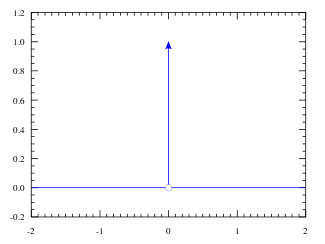
\includegraphics[scale=0.6]{figures/dirac.png}
    \caption{Dirac delta parent function}
\end{figure}

Properties are
\begin{enumerate}
    \item $\int_{a-\epsilon}^{a+\epsilon} \delta(t-a)dt=1$
    \item $\int_{a-\epsilon}^{a+\epsilon} f(t)\delta(t-a)dt=f(a)$
\end{enumerate}

Let $\delta_\tau(t)$ be defined as
\begin{equation*}
    \delta_\tau(t)=\begin{cases}
        \frac{1}{2\tau},-\tau<t<\tau\\
        0, \forall t|t\leq-\tau\land t\geq \tau
    \end{cases}
\end{equation*}

\begin{figure}[H]
    \centering
    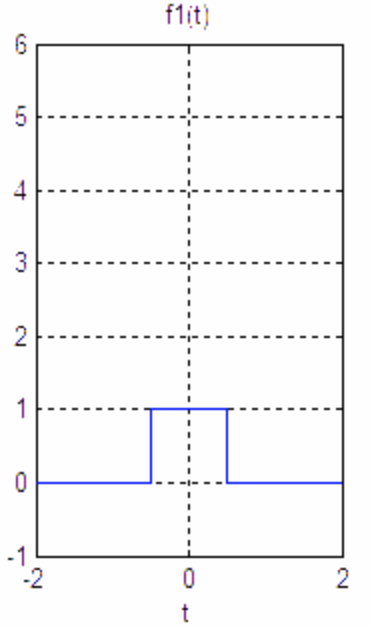
\includegraphics[scale=0.5]{figures/dirac-example.png}
    \caption{Example of $\delta_\tau(t)$}
\end{figure}

Taking the integral,
\begin{equation*}
    \int_{-\infty}^\infty \delta_\tau(t)dt=\int_{-\tau}^\tau \delta_\tau(t)dt=2\tau\left(\frac{1}{2\tau}\right)=1
\end{equation*}

In general, we can state that
\begin{equation*}
    \lim_{\tau\to 0}\delta_\tau(t)=\delta(t)
\end{equation*}
because we are taking the ``rectangle'' base $2\tau\to 0$ but maintaining the area of 1 by making the height $\frac{1}{2\tau}\to \infty$ which is why this value is not arbitrary.

From physics standpoint, works as a sudden impulse and can be used to model such scenarios.
We can multiply by a function, so $f(t)\delta(t-c)$.

\begin{align*}
    \mathcal{L}\{f(t)\delta(t-c)\}&=\int_0^\infty e^{-st}f(t)\delta(t-c)dt\\
    &=\int_{-\infty}^{\infty} e^{-st}f(t)\delta(t-c)dt\\
    &=e^{-sc}f(c)
\end{align*}

The above works because the delta function is scaled by $e^{-st}f(t)$ at $t=c$.